% ENG5027 Assignment 1 report. Each section lives in its own file under sections/ so four
% people can edit at the same time. Figures and code are pulled straight from assignment1/,
% so re-running the scripts updates the report.
\documentclass[11pt,a4paper]{article}

\usepackage[margin=2.3cm]{geometry}
\usepackage[T1]{fontenc}
\usepackage{lmodern}
\usepackage{microtype}
\usepackage{amsmath}
\usepackage{graphicx}
\usepackage{booktabs}
\usepackage{xcolor}
\usepackage{listings}
\usepackage[hidelinks]{hyperref}

\graphicspath{{assignment1/figures/}}

\lstset{
  language=Python,
  basicstyle=\ttfamily\footnotesize,
  keywordstyle=\color{blue!60!black}\bfseries,
  commentstyle=\color{black!55}\itshape,
  stringstyle=\color{green!45!black},
  frame=single, rulecolor=\color{black!15},
  numbers=left, numberstyle=\tiny\color{black!50},
  columns=fullflexible, keepspaces=true,
  showstringspaces=false, breaklines=true,
}

\title{ENG5027 Digital Signal Processing\\Assignment 1: Fourier Transform}
\author{%
  Team 37\\[4pt]
  \begin{tabular}{@{}l l@{}}
    Nommy Khodadad & 3184012K \\
    Parth Sheetal Kumthekar & 3183509K \\
    Abdullah Alkabbawi & 2560946A \\
    Seyedmostafa Hosseini Abardeh & 3184088H \\
  \end{tabular}}
\date{\today}

\begin{document}
\maketitle

% Owner: Abdullah. Two lines only: who, what was recorded, sample rate, equipment.
\section{Introduction}
TODO: speaker, sentence, distances (5\,cm and 1\,m), $f_s$, bit depth, microphone and
software used.

% Owner: A. Reviewer: C.
% Per recording: one time plot, one annotated spectrum (fundamentals, consonant band,
% noise band), 2-3 sentences of reasoning per annotation. Then one paragraph comparing
% 5 cm and 1 m: level, noise floor relative to speech, how much bass is left.
\section{Task 1: time and frequency analysis}

\begin{figure}[h]
  \centering
  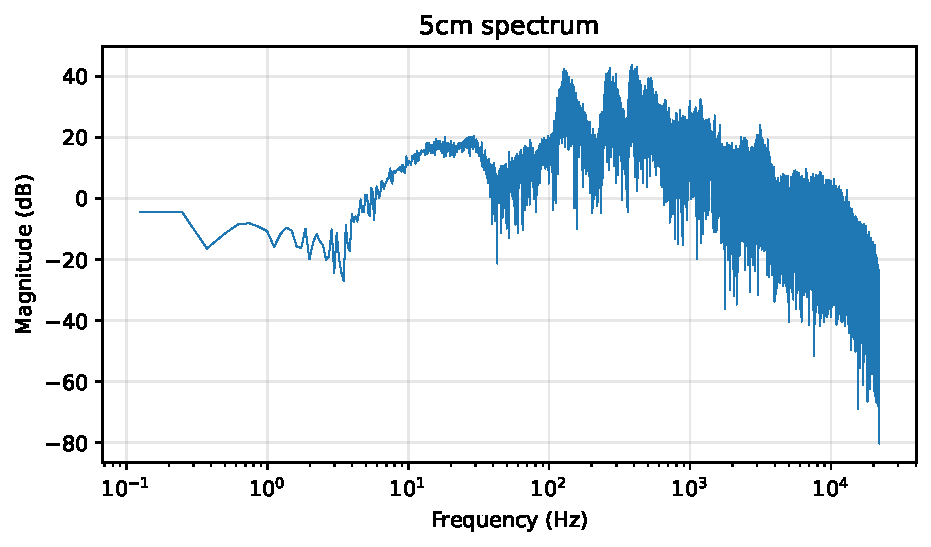
\includegraphics[width=\linewidth]{task1_spectrum_5cm.pdf}
  \caption{Spectrum of the 5\,cm recording. TODO: say what is annotated.}
  \label{fig:t1-spec-5cm}
\end{figure}

TODO

% Owner: Nommy. Reviewer: Seyedmostafa.
% Per recording: noise type and its band; the gain curve with every corner frequency
% justified from the Task 1 plots; before/after spectrum; 1-2 sentences on how it sounds.
% Address bass loss with distance and pops at close range explicitly.
\section{Task 2: enhancement by editing the FFT}

TODO

% Owners: C and D. Reviewers: A and B. Worth 60%.
% v1 and why you started there; each iteration as observed -> changed -> result; the final
% design with its parameters and why you stopped; at least two annotated graphs.
\section{Task 3: aural exciter}

\subsection{Version 1}
TODO

\subsection{Iterations}
\begin{table}[h]
  \centering
  \begin{tabular}{@{}l l l l l p{5cm}@{}}
    \toprule
    Version & Side-chain band & Non-linearity & Drive & Mix & Observed $\to$ changed \\
    \midrule
    v1 & 2--5\,kHz & $\tanh$ & 5 & 0.1 & TODO \\
    v2 &  &  &  &  & TODO \\
    \bottomrule
  \end{tabular}
  \caption{Exciter versions.}
\end{table}

\subsection{Final design}
TODO

% Owner: D. Built from genai-log.md at the end. State which tool (name, version, publisher),
% how it was used, and what the group did itself. Follow the UoG guidance linked in the brief.
\section{GenAI acknowledgement}
TODO


\appendix
\section{Python code}
% Read from assignment1/. When a script changes, upload the new .py over the old one in
% Overleaf so the appendix stays in sync with the code you submit.
\subsection*{audioplot.py (Parts 1 and 2)}
\lstinputlisting{assignment1/audioplot.py}
\subsection*{auralexciter.py (Part 3)}
\lstinputlisting{assignment1/auralexciter.py}

\end{document}
